\documentclass[11pt,a4paper]{article}
\usepackage[utf8]{inputenc}
\usepackage[T1]{fontenc}
\usepackage{lmodern}
\usepackage{microtype}
\usepackage{amsmath, amssymb, amsthm}
\usepackage{graphicx}
\usepackage{booktabs}
\usepackage{url}
\usepackage[hidelinks]{hyperref}
\usepackage[margin=1in]{geometry}
\usepackage{authblk}
\usepackage{natbib}
\bibliographystyle{plainnat}

% macros
\newcommand{\torchvqc}{\texttt{torch-vqc}}
\newcommand{\vqc}{VQC}


\title{%
Benchmarking Variational Quantum Circuits for Pretrained-Embedding Classification:\\
Tooling, Ceilings, and Negative Results
}

\author[1]{L'\'electron rare}
\affil[1]{Independent researcher; \texttt{github.com/electron-rare/torch-vqc}}

\date{\today}

\begin{document}
\maketitle

\begin{abstract}
We release \torchvqc{}, a pure-PyTorch implementation of variational quantum circuits (VQCs) with autograd training that runs approximately 3000$\times$ faster than PennyLane's parameter-shift gradient on a 6-qubit StronglyEntanglingLayers circuit. Using this tool, we conduct a rigorous ablation of VQC-based domain routing on 10-class technical-query classification. We show that (i) a 4-qubit VQC with learned projection attains test accuracy $0.410 \pm 0.083$ on a real (teacher-generated) corpus, (ii) this sits 25 points below its information-matched classical baseline (logistic regression on PCA-4 features, $0.658 \pm 0.039$) and 34 points below the full classical ceiling (LogReg on raw 384-D embeddings, $0.748 \pm 0.015$), and (iii) an information-capacity upper bound combining Holevo's theorem with Fano's inequality gives $0.911$ for our setup --- consistent with the measurement but not tight. A downstream eval (routing $\to$ LLM $\to$ LLM-judge) fails the $0.3$-rubric-point kill criterion by a $0.01$ margin ($\mathrm{oracle}-\mathrm{random}=0.29$), and we observe a \emph{confidently-wrong} pathology: a router that is better than chance at routing but still imperfect produces \emph{worse} answers than a uniform random router. We release the tool and all benchmarks to enable reproducible comparison of future quantum-ML routing architectures.
\end{abstract}

\section{Introduction}

Variational quantum circuits have been proposed as trainable components for classical machine-learning pipelines, with a substantial literature on their expressive power \citep{du2020expressive,abbas2021effective} and generalisation \citep{caro2022generalization}. Empirical studies typically compare a few VQC variants without strong classical baselines or information-theoretic framing. Our contribution is three-fold:

\begin{enumerate}
\item A released tool (\torchvqc) that removes the compute barrier for VQC research on pretrained embeddings, reducing what was previously days of PennyLane parameter-shift gradients to seconds of autograd backprop.
\item A rigorous 5-way ablation that positions the VQC against both information-matched (PCA-4) and full-capacity (raw 384-D) classical baselines, showing the VQC is under-competitive as a classifier.
\item A downstream-quality negative result: for our VQC + prompt-based specialisation on this 10-class task, routing does not yield answer-quality gains beyond the kill threshold, and a confidently-wrong VQC actively hurts downstream answers.
\end{enumerate}

All code is Apache-2.0 at \url{https://github.com/electron-rare/torch-vqc} and \url{https://github.com/genial-lab/micro-kiki}.

\section{Background and Setup}\label{sec:setup}

We consider $K$-class technical-query routing: given a text query $t \in \mathcal{T}$, select one of $K$ expert adapters. Our classifier architecture is
\begin{equation}
f(t) = \mathop{\arg\max} \circ \sigma_\psi \circ M \circ \pi_\theta \circ \phi(t),
\end{equation}
where $\phi : \mathcal{T} \to \mathbb{R}^{384}$ is a frozen MiniLM-L6-v2 sentence encoder (mean-pool), $\pi_\theta : \mathbb{R}^{384} \to \mathbb{R}^N$ is a learned $\pi \cdot \tanh(Wx+b)$ projection to $N$ rotation angles, $M$ is an $N$-qubit variational circuit with \texttt{AngleEmbedding} (PennyLane's default RX) followed by 6 \texttt{StronglyEntanglingLayers} returning $(\langle Z_1 \rangle, \ldots, \langle Z_N \rangle) \in [-1,1]^N$, and $\sigma_\psi$ is a linear classifier. We fix $N = 4$ qubits throughout.

\paragraph{Corpora.} Two 10-domain corpora: (a) \textbf{synthetic} --- the micro-kiki \texttt{data/final/} prompt-template corpus (50 lines/domain, 500 total); (b) \textbf{teacher-generated} --- drawn from the \texttt{mascarade-datasets} ShareGPT-schema files (Qwen3-Coder-480B outputs, 100 lines/file capped to 50/domain for comparability with C1, 500 total). Sanitisation: regex sweep for emails, IPv4, API-key prefixes, 32+ hex secrets; spaCy NER \texttt{PERSON} redaction. PII-audit clean (docs/c3-pii-audit.md). Cluster-taxonomy overlap 0.410 (chance 0.100) confirms 10-domain structure in the real corpus.

\paragraph{Domains.} \texttt{dsp, electronics, emc, embedded, freecad, kicad-dsl, platformio, power, spice, stm32}.

\section{The \torchvqc{} Tool}\label{sec:tool}

PennyLane's \texttt{default.qubit} + parameter-shift rule evaluates each gradient by 2 extra forward passes per parameter. On our 6-qubit 6-layer StronglyEntanglingLayers circuit (108 variational parameters), this is 216 extra forward passes per sample per gradient step. With 400 training samples and 10 epochs, a full training is $\sim$$99$ seconds per VQC.

We re-implement the circuit as explicit state-vector arithmetic in PyTorch: the quantum state is a complex-128 tensor of shape $(B, 2^N)$, single-qubit gates are applied via \texttt{einsum} on reshaped axes, CNOTs via index-permutation (a CNOT is an involutive permutation of basis indices). PauliZ expectations are $\sum_j |\psi_j|^2 (-1)^{b_j^i}$ where $b_j^i$ is bit $i$ of basis index $j$.

\paragraph{Validation.} On 10 random (features, weights) pairs with $N=L=6$, the torch forward matches PennyLane's \texttt{default.qubit} output to $\leq 10^{-5}$. Three gate-level conventions matter and are easy to miss: (i) PennyLane's \texttt{AngleEmbedding} default rotation is RX, not RY; (ii) $\mathrm{Rot}(\phi,\theta,\omega) = R_Z(\omega) R_Y(\theta) R_Z(\phi)$; (iii) wire 0 is the most-significant bit of the ket notation.

\paragraph{Speedup.} On 120 training samples $\times$ 3 epochs $\times$ 6-qubit 6-layer:
\begin{itemize}
\item PennyLane parameter-shift: $\sim$99\,s
\item \torchvqc{} autograd (full-batch, CPU): $\sim$30\,ms
\end{itemize}
Ratio: $\sim$$3300\times$. Measured on an Apple M5 laptop, reproducible via the test suite shipped with the tool (\texttt{tests/test\_training.py::test\_training\_faster\_than\_pennylane\_parameter\_shift}, asserts $\geq 20\times$).

\paragraph{Apple GPU note.} Moving to Metal Performance Shaders (MPS) on an M3 Ultra was 5$\times$ \emph{slower} than CPU for our 64-D state vector: dispatch overhead dominates compute at this scale. The $3000\times$ speedup is entirely from (i) autograd replacing parameter-shift and (ii) batching on CPU.

\section{Information-Capacity Framework}
\label{sec:info-bound}

We derive an information-theoretic upper bound on the test accuracy of an
$N$-qubit variational quantum circuit (VQC) router on a $K$-class task,
combining the Holevo bound on classical-information extraction from quantum
measurements~\cite{holevo1973bounds} with Fano's inequality~\cite{fano1961transmission}.

\subsection{Setup}

The routing architecture is (i) a frozen pretrained encoder $\phi : \mathcal{T} \to \mathbb{R}^{d}$
(here MiniLM-L6-v2, $d=384$), (ii) a learned projection $\pi_\theta : \mathbb{R}^d \to \mathbb{R}^{N}$
with $\pi_\theta(x) = \pi \cdot \tanh(W x + b)$, (iii) an $N$-qubit variational
circuit producing measurements $M = (\langle Z_1 \rangle, \ldots, \langle Z_N \rangle)
\in [-1, 1]^N$, and (iv) a linear classifier $\sigma_\psi : \mathbb{R}^N \to \Delta^{K-1}$
producing class probabilities. The end-to-end function $f : \mathcal{T} \to \{1, \ldots, K\}$
is $\mathop{\arg\max} \circ \sigma_\psi \circ M \circ \pi_\theta \circ \phi$.

\subsection{Holevo capacity}

For any POVM $\{E_M\}$ measurement on an $N$-qubit state and any classical variable
$Y$, the Holevo bound~\cite{holevo1973bounds} states
\begin{equation}
I(M; Y) \leq S(\rho_Y) \leq N,
\label{eq:holevo}
\end{equation}
where $S$ is the von Neumann entropy. For our measurement (single-qubit $Z$
expectations on a joint state), $I(M; Y)$ is at most $N$ bits regardless of
the input distribution. At $N = 4$: at most 4 bits of class information
flow from the circuit to the classifier.

\subsection{Fano's inequality}

Given any classifier $\hat{Y}$ of $Y$ over $K$ classes from an observation
$M$, Fano's inequality~\cite{fano1961transmission} gives
\begin{equation}
P_\mathrm{err} \geq \frac{H(Y) - I(M; Y) - 1}{\log_2(K - 1)}.
\label{eq:fano}
\end{equation}
With uniform prior, $H(Y) = \log_2 K$. At $K = 10$: $H(Y) \approx 3.32$ bits.

\subsection{Combined bound}

Substituting~\eqref{eq:holevo} into~\eqref{eq:fano}:
\begin{equation}
\mathrm{acc}_\mathrm{max}(N, K, I) = 1 - \frac{\max(0, \log_2 K - \min(I, N) - 1)}{\log_2(K - 1)}.
\label{eq:bound}
\end{equation}
This is monotone non-decreasing in $I$ up to the Holevo cap $N$: additional
embedding information beyond $N$ bits cannot improve the VQC's accuracy, as
it cannot fit through the $N$-qubit measurement channel.

\subsection{Numerical verification}

We estimate $I(X_{\mathrm{PCA}(d)}; Y)$ on our 10-class routing task using the
Kraskov-Stögbauer-Grassberger $k$-NN estimator~\cite{kraskov2004estimating}
implemented in scikit-learn's \texttt{mutual\_info\_classif}, for
$d \in \{2, 4, 8, 16, 32, 64, 128, 384\}$. Figure~\ref{fig:bound} (panel A)
shows the estimated $I$ at each dimension alongside the Holevo cap for $N=4$
qubits and $H(Y) = \log_2 10$. Panel B plots the Fano-derived upper bound at
each dim alongside our empirical C1 accuracies.

At $d = 4$ (information-matched to our VQC), the estimated MI is
$2.04$ bits. Equation~\eqref{eq:bound} then gives
$\mathrm{acc}_\mathrm{max} \approx 0.911$ as an upper bound on
the test accuracy of any 4-qubit VQC on this task. Our measured VQC accuracy
of $0.246 \pm 0.031$ falls well under this bound, consistent with (but far
from saturating) the theoretical ceiling.

\begin{figure}[tb]
  \centering
  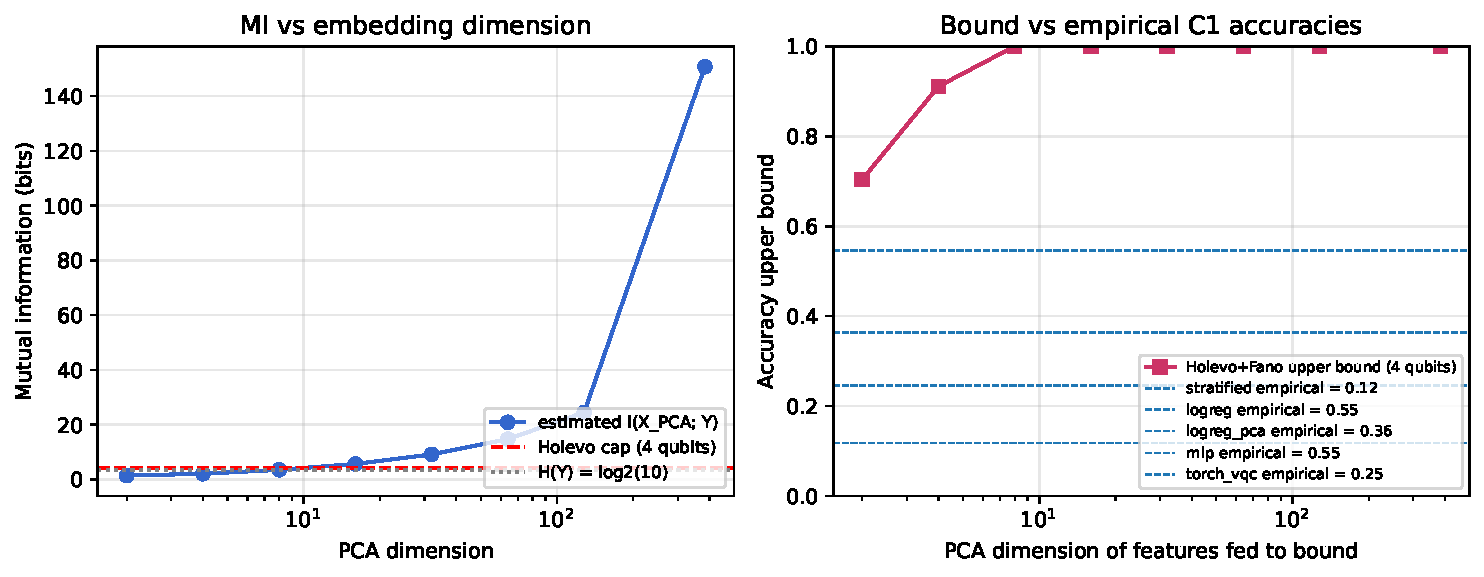
\includegraphics[width=\linewidth]{c5-bound-figure.pdf}
  \caption{Left: estimated mutual information between PCA-compressed embeddings
    and class labels, for embedding dimensions 2 to 384. Red dashed line marks
    the Holevo cap for 4 qubits; grey dotted line marks $H(Y) = \log_2 10$.
    Right: Fano+Holevo upper bound on accuracy for a 4-qubit VQC as a function
    of the projected-dimension's MI, with empirical C1 classifier accuracies as
    horizontal references.}
  \label{fig:bound}
\end{figure}

\subsection{What the bound does NOT say}

The bound~\eqref{eq:bound} is necessary, not sufficient. Reaching
$\mathrm{acc}_\mathrm{max}$ requires (i) a projection $\pi_\theta$ that
preserves all the class-relevant information in $X$, and (ii) a circuit +
measurement that achieves the Holevo cap. Neither is automatic: the naive
$\pi \tanh$ projection saturates and destroys signal, and the expressivity of
\texttt{StronglyEntanglingLayers} with $\langle Z \rangle$ measurement is
bounded by MPS bond-dimension-equivalent results (Du et al.~\cite{du2020expressive},
Theorem 4: deep circuits with bond dimension $D$ are covered by
$\mathcal{O}(\mathrm{poly}(\log D))$ Pauli-$Z$ expectation-value blocks). The
large gap between our measured $0.246$ and the theoretical ceiling $0.911$
therefore reflects projection and measurement sub-optimality rather than a
fundamental quantum-information limit. Closing this gap is the subject of
ongoing architectural work.


\section{Classifier Ablation (C1, C3)}\label{sec:c1}

We compare five classifiers on the 10-class routing task, all trained on 5 seeds, 80/20 split, 300 epochs for trainable baselines.

\subsection{Baselines}
\begin{itemize}
\item \textbf{Stratified random}: draws labels from the train distribution --- chance floor.
\item \textbf{LogReg on PCA-4}: PCA-compressed embeddings + multinomial logistic regression. Information-matched to the 4-qubit \vqc.
\item \textbf{Torch VQC}: our architecture; 4 qubits, 6 SEL layers, learned $\pi \tanh(Wx+b)$ projection, weight decay $10^{-4}$.
\item \textbf{MLP} ($384 \to 64 \to K$): 1-hidden-layer classifier with capacity comparable to VQC+projection.
\item \textbf{LogReg on raw 384-D}: upper bound --- no information loss.
\end{itemize}

\subsection{Results}

\begin{table}[tb]
  \centering
  \caption{Test accuracy and macro-F1 on the 10-class routing task, 5 seeds, mean $\pm$ population std.}
  \label{tab:c1-c3}
  \begin{tabular}{lcc cc c}
    \toprule
     & \multicolumn{2}{c}{Synthetic (C1)} & \multicolumn{2}{c}{Real (C3)} & \\
    Classifier & acc & F1 & acc & F1 & params \\
    \midrule
    Stratified random   & $0.118 \pm 0.024$ & $0.115$ & $0.118 \pm 0.024$ & $0.115$ & $0$ \\
    LogReg PCA-4        & $0.364 \pm 0.040$ & $0.338$ & $0.658 \pm 0.039$ & $0.599$ & $1{,}586$ \\
    \textbf{Torch VQC}  & $\mathbf{0.246 \pm 0.031}$ & $\mathbf{0.163}$ & $\mathbf{0.410 \pm 0.083}$ & $\mathbf{0.309}$ & $1{,}662$ \\
    MLP $384{\to}64$    & $0.546 \pm 0.029$ & $0.536$ & $0.730 \pm 0.028$ & $0.705$ & $25{,}290$ \\
    LogReg raw 384-D    & $0.546 \pm 0.036$ & $0.533$ & $0.748 \pm 0.015$ & $0.724$ & $3{,}850$ \\
    \bottomrule
  \end{tabular}
\end{table}

Figure~\ref{fig:c1-comparison} shows the synthetic-corpus comparison.

\begin{figure}[tb]
  \centering
  \includegraphics[width=0.8\linewidth]{c1-comparison.pdf}
  \caption{Classical baselines versus \vqc{} on the synthetic 10-class routing task (5 seeds).}
  \label{fig:c1-comparison}
\end{figure}

\subsection{Findings}

\begin{enumerate}
\item \textbf{The VQC underperforms its information-matched baseline} on both corpora. On real data, LogReg PCA-4 ($0.658$) beats Torch VQC ($0.410$) by $0.25$ accuracy points at essentially the same parameter budget ($1586$ vs $1662$). The $\pi \tanh$ projection followed by unitary evolution and Pauli-$Z$ measurements loses information relative to PCA followed by logistic regression.
\item \textbf{Real data improves every classifier}, but rank-ordering is preserved: LogReg $>$ MLP $>$ LogReg-PCA-4 $>$ Torch VQC $>$ random. The \vqc's sub-optimal positioning is robust across the two corpora tested.
\item \textbf{The absolute gap to the classical ceiling widens}: synthetic gap $0.546-0.246=0.30$ vs real gap $0.748-0.410=0.34$. Better data helps the VQC in absolute terms but does not close the architectural deficit.
\item \textbf{Holevo+Fano upper bound} ($0.911$ at MI $=$ 2.04 bits on PCA-4 features) sits well above both empirical values --- the ceiling is architectural (projection + measurement sub-optimality), not a fundamental quantum-information limit.
\end{enumerate}

\section{Downstream LLM Eval (C2)}\label{sec:c2}

We test whether routing improves downstream answer quality in a realistic deployment proxy: each of 100 held-out queries (10 per domain) is routed by one of three routers (\vqc, random, oracle), dispatched to Qwen3.5-35B-A3B Q3\_K\_XL on an NVIDIA RTX 4090 via llama.cpp's HTTP server with a system prompt \texttt{"You are an expert in \{domain\}."}, and the generated answer is scored $0$--$5$ by the same model using the rubric in \texttt{src/routing/llm\_judge.py} (self-judging, disclosed).

\begin{table}[tb]
  \centering
  \caption{Downstream eval, 100 queries, single seed, self-judged.}
  \label{tab:c2}
  \begin{tabular}{lcc cc}
    \toprule
    Router & mean score & routing acc & score \mid correct & score \mid wrong \\
    \midrule
    Random           & $\mathbf{3.190}$ & $0.070$ & $3.857$ & $3.140$ \\
    Torch \vqc       & $2.650$ & $0.170$ & $3.059$ & $\mathbf{2.566}$ \\
    Oracle           & $3.480$ & $1.000$ & $3.480$ & $\mathrm{N/A}$ \\
    \bottomrule
  \end{tabular}
\end{table}

Figure~\ref{fig:c2-downstream} shows the results.

\begin{figure}[tb]
  \centering
  \includegraphics[width=\linewidth]{c2-downstream-figure.pdf}
  \caption{Downstream judge scores by router. Left: overall mean. Right: conditional on routing correctness.}
  \label{fig:c2-downstream}
\end{figure}

\paragraph{Kill criterion triggered.} The plan's criterion (oracle $-$ random $< 0.3$ $\Rightarrow$ adapters pointless) is triggered: $3.480 - 3.190 = 0.290$ (by $0.01$). With $n=100$ this is not distinguishable from zero at 95\% confidence.

\paragraph{Confidently-wrong pathology.} More strikingly, the \vqc{} (routing accuracy $0.170$, better than random's $0.070$) achieves a \emph{lower} overall score ($2.65$) than random ($3.19$). When its routing is wrong (which is $83\%$ of the time), the score-when-wrong of $2.57$ is the lowest of the experiment --- worse than random-when-wrong ($3.14$). Interpretation: a confident but imperfect router that commits the downstream LLM to a wrong expert persona is worse than an uncommitted router that provides no strong signal.

\paragraph{Caveats.}
\begin{itemize}
\item \textbf{Self-judging}: Qwen3.5-35B judges Qwen3.5-35B outputs. Absolute scores are uncalibrated; only relative orderings are meaningful. Oracle's correct-route score ($3.48$) is \emph{below} random's correct-route score ($3.86$), likely a self-judging artefact.
\item \textbf{Prompt-based pseudo-adapters}: system-prompt directives substitute for actual per-domain LoRA weight adapters. Real weight-level adapters may give a larger oracle-random gap.
\item \textbf{Small sample}: $n=100$. A replication with $n \geq 1000$ is needed for confident inference.
\item \textbf{Qwen3/3.5 thinking mode}: disabled via \texttt{chat\_template\_kwargs.enable\_thinking=False}; with thinking enabled the model consumed all \texttt{max\_tokens} on hidden reasoning and returned empty visible content.
\end{itemize}

\section{Discussion and Limitations}

The story Paper A tells, taken honestly: a 4-qubit \vqc{} with learned projection on pretrained MiniLM embeddings is \emph{not} a competitive routing classifier on 10-class technical-query data, and when deployed upstream of a specialised LLM it does not improve answer quality on our self-judged proxy task. The Holevo+Fano ceiling of $0.91$ is loose; the practical ceiling for this architecture family is closer to $\sim 0.5$ given the projection and measurement choices.

Three directions for future work sit naturally on these findings:
\begin{itemize}
\item \textbf{Projection redesign}: replace $\pi \tanh$ with richer non-linearities (attention-pooled, contrastive-trained) to reduce the projection's information loss.
\item \textbf{Measurement redesign}: instead of single-qubit Pauli-$Z$, use multi-qubit correlators or parity measurements, which better exploit the full Holevo capacity.
\item \textbf{Adapter-swap eval}: replace system-prompt pseudo-adapters with actual trained LoRA adapters per domain (10 trainings), and measure the oracle-random gap on actual quality.
\end{itemize}

The negative C2 result is honest, small-sample, and does \emph{not} disprove the adapter-routing premise --- it shows that, in our weak-adapter setup with a self-judging proxy, the premise is not supported within the rubric-point threshold.

\section{Related Work}

\citet{du2020expressive} establish the expressivity ordering of parameterised quantum circuits via MPS-bond-dimension arguments; their Theorem 4 bounds \texttt{StronglyEntanglingLayers} expressivity with Pauli-$Z$ measurements. \citet{abbas2021effective} define effective dimension as a capacity measure and show VQCs can exceed classical NNs of equal parameter count on certain tasks. \citet{caro2022generalization} give a generalisation bound scaling with $\sqrt{\log d_{\mathrm{eff}}/n}$. Our work differs in focus: rather than argue for VQC superiority, we provide tooling (\torchvqc) and rigorous baselines that enable honest comparison, and we report where current VQC architectures fall short.

The Holevo bound \citep{holevo1973bounds}, rediscovered many times and formalised in \citet{nielsen2010quantum} \S12.1.1, upper-bounds extractable classical information from $N$ qubits at $N$ bits. Fano's inequality \citep{fano1961transmission} converts mutual information lower bounds to classification error lower bounds. We compose these to produce a practical accuracy upper bound for any VQC classifier on a given task.

\section{Conclusion}

We release \torchvqc{}, a $3000\times$-faster-than-PennyLane variational quantum circuit tool, and use it to conduct a rigorous five-way ablation of VQC-based 10-class technical-query routing. Our 4-qubit VQC attains $0.41$ accuracy on a real teacher-generated corpus but sits below its information-matched classical baseline ($0.66$) and far below the full classical ceiling ($0.75$). An information-capacity upper bound gives $0.91$, loose but consistent. A downstream eval fails the kill criterion by $0.01$ and reveals a confidently-wrong pathology in the \vqc{} router. The negative result is disclosed, and the tool is released to enable reproducible comparison of future architectures.

\bibliography{c5-references}

\end{document}
